% !TEX encoding = UTF-8 Unicode
%\documentclass[twoside]{article}
\documentclass[twocolumn,10pt]{article}
\usepackage[french]{babel}
\usepackage[utf8]{inputenc}
\usepackage[T1]{fontenc}

\usepackage{amsmath}
\usepackage{amssymb}
\usepackage{amsfonts}
\usepackage{graphicx}
%\usepackage{bbm}

\usepackage[margin=2cm,top=32mm,columnsep=20pt]{geometry}
\usepackage{multirow,multicol} % Style double colonne 
\usepackage{abstract} % Customization de l'abstract 
\usepackage{fancyhdr} % en-têtes et pieds de page 
\usepackage{float} % Nécessaire pour les tables et figures dans l'environnement double colonne 

\usepackage{url}
\usepackage[colorlinks=true,linkcolor=red,urlcolor=blue,filecolor=green,citecolor=red]{hyperref} % hyperliens 
\usepackage{dtk-logos}

\usepackage[ddmmyyyy]{datetime}

\newdateformat{ddmmyyyy}{\twodigit{\THEDAY}/\twodigit{\THEMONTH}/\THEYEAR\xspace}

\def\currentyear{\the\year}
\newdate{revuedeb}{21}{04}{\currentyear}
\newdate{revuefin}{26}{04}{\currentyear}
\newdate{soutdeb}{15}{06}{\currentyear}
\newdate{soutfin}{20}{06}{\currentyear}

% En-têtes et pieds de page 
\pagestyle{fancy}  
\fancyhead{} % Blank out the default header
\fancyfoot{} % Blank out the default footer
\fancyhead[C]{Projets de SY09} % Custom header text
\fancyfoot[RO,LE]{\thepage} % Custom footer text

\setlength{\parskip}{1ex} % espace entre paragraphes 

%\renewcommand{\arraystretch}{1.5} % plus d'espace dans les tableaux 
\usepackage{booktabs} % pour de plus beaux tableaux 
\usepackage{caption} % gestion des légendes 
\captionsetup[table]{skip=10pt} % espacement recommandé 

% environnement de propriétés 
\newtheorem{propriete}{Propriété}
\newtheorem{remarque}{Remarque}

% symboles mathématiques 
\newcommand{\calN}{\mathcal{N}}
\newcommand{\bsx}{\boldsymbol{x}}
\newcommand{\bsX}{\boldsymbol{X}}
\newcommand{\bsxa}{\boldsymbol{x}_{{A}}}
\newcommand{\bsXa}{\boldsymbol{X}_{{A}}}
\newcommand{\bsxb}{\boldsymbol{x}_{{B}}}
\newcommand{\bsXb}{\boldsymbol{X}_{{B}}}
\newcommand{\bsmu}{\boldsymbol{\mu}}
\newcommand{\bsSig}{\boldsymbol{\Sigma}}
\newcommand{\bsmua}{\boldsymbol{\mu}_{{A}}}
\newcommand{\bsmub}{\boldsymbol{\mu}_{{B}}}
\newcommand{\bsSigaa}{\boldsymbol{\Sigma}_{AA}}
\newcommand{\bsSigab}{\boldsymbol{\Sigma}_{AB}}
\newcommand{\bsSigba}{\boldsymbol{\Sigma}_{BA}}
\newcommand{\bsSigbb}{\boldsymbol{\Sigma}_{BB}}
\newcommand{\transp}[1]{{#1}^\top}


%----------------------------------------------------------------------------------------

\title{Projets en groupe --- printemps \the\year}

\author{Benjamin Quost}
\date{\today}

\begin{document}

\maketitle % Insert title
\thispagestyle{fancy} % All pages have headers and footers

\begin{abstract}

Vous avez un projet à réaliser au cours de l'UV, en groupes, qui a une double vocation pédagogique et d'évaluation. Il a pour objectif d'appliquer les méthodes étudiées au cours du semestre sur des jeux de données réelles. Vous rendrez compte du travail effectué et de la démarche adoptée lors d'une soutenance sur la base d'un poster; vous vous appuierez également sur un bref rapport, qui ne sera pas évalué mais vous permettra de donner des précisions sur votre travail. 

Ce document précise les modalités du projet (conditions de réalisation et d'évaluation), donne quelques conseils généraux pour le bon déroulement de votre travail, et fournit quelques indications sur la rédaction du rapport. 
Celui-ci, \emph{qui n'excèdera pas quatre pages} (en style \frquote{double-colonne}), sera rédigé en \LaTeX{}. Vous pouvez réutiliser le fichier source du présent document. Un premier rendu intermédiaire sera fait peu avant la revue de projet à mi-parcours. La version finale sera rendue avant les soutenances. 

\end{abstract}


%----------------------------------------------------------------------------------------

\section*{Introduction}

Ce document présente les conditions de réalisation du projet de SY09 pour le semestre de printemps \the\year. 

Le document présente tout d'abord (en partie~\ref{sec:proj}) les modalités de réalisation du projet, les livrables à fournir, et les conditions d'évaluation. Le travail sera réalisé en groupes; il portera sur l'analyse et le traitement d'un jeu de données, \emph{choisi avec soin} par le groupe. Le travail réalisé sera restitué lors d'une soutenance en fin de semestre, sur la base d'un poster; des éléments complémentaires pourront être donnés dans un rapport. 

Ce rapport fera l'objet d'un rendu, avant les soutenances de projets. Il ne sera pas évalué, mais vous permettra de donner des compléments d'information sur votre travail: il est donc particulièrement important pour la mise en valeur de ce dernier. 
Pour cette raison, ce document donne (en partie~\ref{sec:CR}) quelques conseils pour la rédaction de rapports de qualité. 


%----------------------------------------------------------------------------------------

\section{Modalités du projet}\label{sec:proj}

Cette première partie donne des précisions sur le choix des jeux de données, le calendrier du projet, et l'évaluation du travail réalisé par les groupes. 


%-------------------------------------------------

\subsection{Groupes et choix des données}\label{subsec:proj:groupes}

Le travail sera réalisé en groupes de trois personnes, tirés au hasard. 
Chaque groupe travaillera tout au long du semestre sur un même jeu de données, mis à disposition par l'équipe enseignante. 
Les groupes sont autorisés à choisir un jeu de données provenant d'une autre source, à condition que le choix ait été validé par l'équipe enseignante. 


%-------------------------------------------------

\subsection{Travail à réaliser}\label{subsec:proj:travail}

L'objectif est d'analyser le jeu de données \href{https://www.kaggle.com/datasets/uciml/student-alcohol-consumption}{\texttt{Student Alcohol Consumption}}, disponible sur Kaggle. 

Le projet est volontairement peu cadré: les données sont riches, et peuvent faire l'objet de différentes analyses (différents traitements pour mettre en évidence différents effets). Les groupes seront évalués sur leur capacité à appliquer les méthodes étudiées en SY09\footnote{Les méthodes non étudiées en cours ne sont pas exigibles.}. 

L'évaluation dépendra en grande partie de la cohérence dans les différentes analyses. La maîtrise des outils et l'originalité des analyses seront également prise en compte: le plagiat (codes ou travaux) et l'incapacité à expliquer des résultats obtenus ou montrés en soutenance seront sanctionnés. L'originalité des analyses réalisées pourra être prise en compte. 


%-------------------------------------------------

\subsection{\'Evaluation}\label{subsec:proj:eval}

\paragraph{Soutenances}

Le travail réalisé sera restitué par le groupe lors d'une soutenance, sur la base d'un poster ou de transparents --- nous donnerons davantage d'informations sur ce point dans le courant du semestre. 

Seule la prestation orale, évaluée lors d'une soutenance entre le \displaydate{soutdeb} et le \displaydate{soutfin}, sera notée. Néanmoins, le temps imparti à chaque groupe étant limité, chaque groupe pourra s'appuyer sur un rapport, qui constituera un complément d'information sur le travail réalisé. 

\paragraph{Individualisation de l'évaluation}

Il est important que chaque membre d'un groupe ait une maîtrise raisonnable de l'\emph{ensemble des travaux réalisés} par le groupe et présentés lors de la soutenance. Nous veillerons à évaluer ce point lors des soutenances. 

L'équipe enseignante pourra ainsi poser des questions ciblées à chaque membre d'un groupe, de manière à évaluer son niveau d'implication et à juger de sa maîtrise des notions étudiées en SY09. Les réponses à ces questions détermineront en partie la note du projet, qui pourra donc être différente pour les membres d'un même groupe. 


%----------------------------------------------------------------------------------------

\section{Rapports}\label{sec:CR}

Cette partie donne quelques conseils de réalisation des rapports de projets. Ces derniers ne seront pas évalués, mais permettent de communiquer des éléments complémentaires qu'il serait difficile de développer lors de la soutenance et de mettre en valeur les travaux réalisés: il est donc important d'en soigner la réalisation. 

%-------------------------------------------------

\subsection{Introduction}\label{subsec:CR:intro}

Le document doit être concis, c'est-à-dire suffisamment synthétique sans pour autant omettre d'informations importantes. Il devra être rédigé avec \LaTeX{}, dans le style du document présent (dont vous pourrez reprendre le code source), et ne devra pas excéder quatre pages (style double colonne). 

Le document pourra respecter la structure suivante: 
\begin{enumerate}
\item une introduction, rappelant la problématique (présentation brève des données, questions auxquelles le travail cherche à répondre, plan); 
\item une partie principale, articulée suivant la problématique d'étude, pouvant contenir différentes parties: présentation des données, puis des différentes analyses effectuées; 
\item une conclusion, résumant les résultats principaux et présentant d'éventuelles perspectives dont la mise en \oe{}uvre dépasse le cadre du TP. 
\item D'éventuelles annexes pourront contenir le code, les figures (si elles sont trop nombreuses pour être mises dans le texte), voire des détails de calculs un peu longs. 
\end{enumerate}

Nous donnons ci-dessous quelques conseils généraux sur le contenu d'un rapport (partie~\ref{subsec:CR:contenu}) et sur sa forme (partie~\ref{subsec:CR:forme}). La restitution de formules mathématiques est abordée au paragraphe~\ref{subsubsec:CR:maths}, de code au paragraphe~\ref{subsubsec:CR:code}, et de tableaux ou de figures au paragraphe~\ref{subsubsec:CR:figures}. 
La question de la bibliographie est brièvement traitée au paragraphe~\ref{subsec:CR:biblio}. 

\begin{remarque}[\LaTeX{}]
Nous imposons l'usage de \LaTeX{}, car cette solution logicielle riche, performante, libre et gratuite, permet d'élaborer des documents de qualité. L'usage de \LaTeX{} ne garantit pas la qualité du document final (le respect des bonnes pratiques de rédaction revient aux auteurs d'un document), mais la favorise néanmoins, pour plusieurs raisons: 
\begin{itemize}
\item l'utilisation de balises incite à dissocier le contenu de la mise en page, qui est très facile à modifier (comme par exemple le choix du style \frquote{double colonne} dans l'en-tête du document); 
\item cela permet une grande flexibilité dans la manipulation du contenu (paragraphes, figures, tableaux, algorithmes, équations, etc), même en modifiant la structure du rapport; 
\item la gestion des équations (et des écritures mathématiques en général), ainsi que du code, est particulièrement aisée. 
\end{itemize}
La mise en page est rigoureuse, et respecte par défaut les règles d'usage en typographie: on en tire donc en général de beaux documents, plus faciles à lire. 

Le prix à payer est d'investir un peu d'énergie pour découvrir \LaTeX{}. Ce n'est pas si difficile, et le retour sur investissement est rapide et conséquent. L'existence d'une documentation très abondante et de fichiers types rend la tâche encore plus aisée. Un manuel très complet est disponible en ligne \cite{oetiker18} (une version française, plus ancienne, est disponible par exemple \href{https://ctan.org/tex-archive/info/lshort/french}{à cette URL}). 
\end{remarque}


%-------------------------------------------------

\subsection{Contenu du rapport}\label{subsec:CR:contenu}

L'analyse des résultats obtenus lors de votre travail sera effectuée lors de la soutenance. \'Etant donné le peu temps disponible pour cette présentation orale, il vous est recommandé de détailler votre travail dans un rapport que vous pourrez utiliser comme support. Ce rapport devant être succinct (quatre pages double colonne), il devra en conséquence être soigneusement élaboré pour avoir une réelle valeur ajoutée. 

Le rapport vous permettra de préciser les choix faits lors du traitement du jeu de données que vous avez choisi, et de préciser le cheminement intellectuel qui vous a conduit aux résultats présentés lors de la soutenance. Les méthodes ou algorithmes utilisés peuvent être décrits succinctement. Le code source devrait être évité dans le rapport, à moins qu'ils ne présente un intérêt particulier; il peut être consigné en annexe, pour ne pas perturber la lecture. 


%-------------------------------------------------

\subsection{Forme}\label{subsec:CR:forme}

Nous donnons ci-dessous quelques conseils généraux sur la forme du rapport, concernant la mise en page et le choix des polices, la présentation de résultats formels (mathématiques), techniques (algorithmes), ou graphiques (tableaux, figures). 


%---------------------

\subsubsection{Police et mise en page}\label{subsubsec:CR:miseenpage}

Un bon document doit être sobre: les fioritures fatiguent à long terme le lecteur. N'abusez pas d'effets de style. On évitera l'usage de caractères gras ou d'une police soulignée: pour mettre en valeur un élément de texte, on utilisera l'\emph{italique}. Adoptez un \frquote{code graphique} cohérent et simple, en n'utilisant qu'un seul effet de style pour une seule signification. 

Les changements de taille ou de style de police nuisent à l'harmonie graphique du document, et sont donc à proscrire. On pourra faire une exception à cette règle dans des cadres bien spécifiques, par exemple en utilisant le gras pour distinguer les vecteurs des variables, ou une police particulière pour écrire du code (paragraphes \ref{subsubsec:CR:maths} et \ref{subsubsec:CR:code}). 

Un document rédigé en pleine page (\frquote{simple colonne}) est plus agréable à lire que présenté sur deux colonnes, mais prend plus de place: si le nombre de pages est contraint, le style \frquote{double colonne} est préférable. 
Inutile de rajouter des sauts de ligne ou des espaces, \LaTeX{} fait ça très bien tout seul. N'abusez pas des notes de bas de page\footnote{Les notes de bas de page sont plutôt dévolues aux apartés; mal utilisées, elles gênent la lecture en en brisant le fil.}, qui fractionnent la lecture; les précisions doivent rester dans le corps du texte (par exemple entre parenthèses), ou être développées dans un paragraphe à part. 


%---------------------

\subsubsection{Mathématiques}\label{subsubsec:CR:maths}

L'un des nombreux avantages de \LaTeX{} est la simplicité de rédaction et de gestion des formules mathématiques. Vous pouvez ainsi insérer des équations seules, comme c'est le cas pour l'équation \eqref{eqn:poly2-1D}: 
\begin{equation}\label{eqn:poly2-1D}
f(x) = a x^2 + b x + c , 
\end{equation}
ou des suites d'équations (alignées, pour plus de clarté) comme les équations \eqref{eqn:poly2-2D-1}-\eqref{eqn:poly2-2D-2}: 
\begin{align}
\label{eqn:poly2-2D-1} f(\bsx) & = \transp{\bsx} A \bsx + \transp{b} \bsx + c , \\ 
\label{eqn:poly2-2D-2} \text{t.q. } \bsx & \in \mathbb{R}^2 , 
\end{align}
où $A$ et $b$ sont définis par: 
\begin{equation*}
%\bsx = \left(\begin{array}{cc}
%x_1 \\ 
%x_2 
%\end{array}\right) , 
%\quad 
A = \left(\begin{array}{cc}
a_{11} & a_{12} \\ 
a_{21} & a_{22} 
\end{array}\right) , 
\quad 
b = \left(\begin{array}{cc}
b_1 \\ 
b_2 
\end{array}\right) . 
\end{equation*}
Remarquons que cette dernière équation n'a pas été étiquetée: on ne peut pas y faire référence (sauf avec une périphrase, ce qui nuit à la concision du propos). 
Une équation longue (comme l'équation~\eqref{eqn:poly2-2D-dev}) peut figurer sur plusieurs lignes: 
\begin{multline}
\label{eqn:poly2-2D-dev} f(x_1,x_2) = a_{11} x_1^2 + a_{22} x_2^2 + a_{21} x_1 x_2 \\ + a_{12} x_1 x_2 + b_1 x_1 + b_2 x_2 . 
\end{multline}
Les développements mathématiques complexes ou d'intérêt secondaire doivent autant que possible figurer dans un paragraphe à part ou en annexe, pour ne pas gêner la lecture (voir par exemple l'annexe~\ref{ann:gaus}). 

Remarquons que \LaTeX{} offre la possibilité de définir des commandes pour les usages répétés, comme par exemple pour les symboles \frquote{$\bsx$} et \frquote{$\transp{}$} (voir l'en-tête du fichier source de ce document). Pour plus de renseignements, on pourra se reporter à \cite{oetiker18} (ou à la version française, plus ancienne). 


%---------------------

\subsubsection{Algorithmes et code source}\label{subsubsec:CR:code}

Comme nous l'avons dit plus haut, le corps du texte ne devrait pas comporter de code source complexe, comme des fonctions ou des scripts: cela nuit au confort de lecture et à la clarté du document. La mention d'un petit nombre de commandes, si nécessaire, est tolérable. Le code plus complexe peut être consigné en annexe. 

Si vous avez développé un algorithme particulier pour effectuer un traitement spécifique sur des données, il vous est possible de le présenter de manière formelle (de préférence en annexe) et d'y faire référence grâce à un environnement adapté, comme celui fourni par le package \LaTeX{} \verb?algorithm2e?. 


%---------------------

\subsubsection{Tableaux et figures}\label{subsubsec:CR:figures}

D'une manière générale, les informations communiquées dans le rapport doivent être lisibles et informatives. Les tableaux et les figures peuvent vous y aider. Nous rappelons ici quelques règles de bon sens. 

\LaTeX{} permet de créer des tableaux et des figures assez facilement, pour ensuite y faire référence dans votre rapport. Vous trouverez des exemples dans ce document, avec le tableau~\ref{tab:exemple} et les figures \ref{fig:iris1} et \ref{fig:iris2}. 

La disposition des tableaux et figures (appelés \frquote{objets flottants}) peut être délicate lors de la rédaction d'un document: la compilation peut les positionner dans des endroits peu désirables. 
Il peut être nécessaire de tâtonner en positionnant le code correspondant à différents endroits dans le code source du document (et en recompilant à chaque fois) jusqu'à obtenir une configuration satisfaisante. 

%% Tableau "classique" 
%\begin{table}[htbp]
%\begin{center}
%\caption{\label{tab:exemple}Exemple de tableau.}
%\begin{tabular}{ccc}
%UV & niveau & remarque \\
%\hline
%SY02 & branche & classe \\
%SY09 & filière & top \\
%SY19 & filière & très bien \\ 
%\end{tabular}
%\end{center}
%\end{table}

% Tableau package booktabs 
\begin{table}[htbp]
\begin{center}
\caption{\label{tab:exemple}Exemple de tableau.}
\begin{tabular}{ccc}
\toprule
UV & niveau & remarque \\
\midrule
SY02 & branche & classe \\
SY09 & filière & top \\
SY19 & filière & très bien \\ 
\bottomrule
\end{tabular}
\end{center}
\end{table}

On évitera d'afficher trop de tableaux ou de figures. Ceux qui seront affichés devront être \frquote{optimisés} de manière à communiquer autant d'informations \emph{pertinentes} que possible en un minimum de place. Il faut éviter les tableaux ou figures \frquote{orphelins} (sans légende, pas numérotés, sans référence). La légende, synthétique (le texte doit contenir l'essentiel de l'information), doit permettre au lecteur de situer la figure par rapport au corps du texte. Par convention, la légende se met en haut pour un tableau et en bas pour une figure. 

On apportera une attention particulière à la lisibilité: éviter les valeurs avec trop de chiffres significatifs, utiliser un style épuré (comme pour le tableau~\ref{tab:exemple}, défini avec un minimum de lignes séparatrices). On n'oubliera pas d'indiquer les échelles sur les graphiques, d'étiqueter les axes, etc. 
Les couleurs et les symboles permettent d'ajouter une information supplémentaire parfois précieuse (par exemple, l'espèce d'iris, sur la figure~\ref{fig:iris1} qui représente les données collectées par Anderson \cite{anderson35} et popularisées par Fisher \cite{fisher36}). 

\begin{figure}[htbp]
\begin{center}
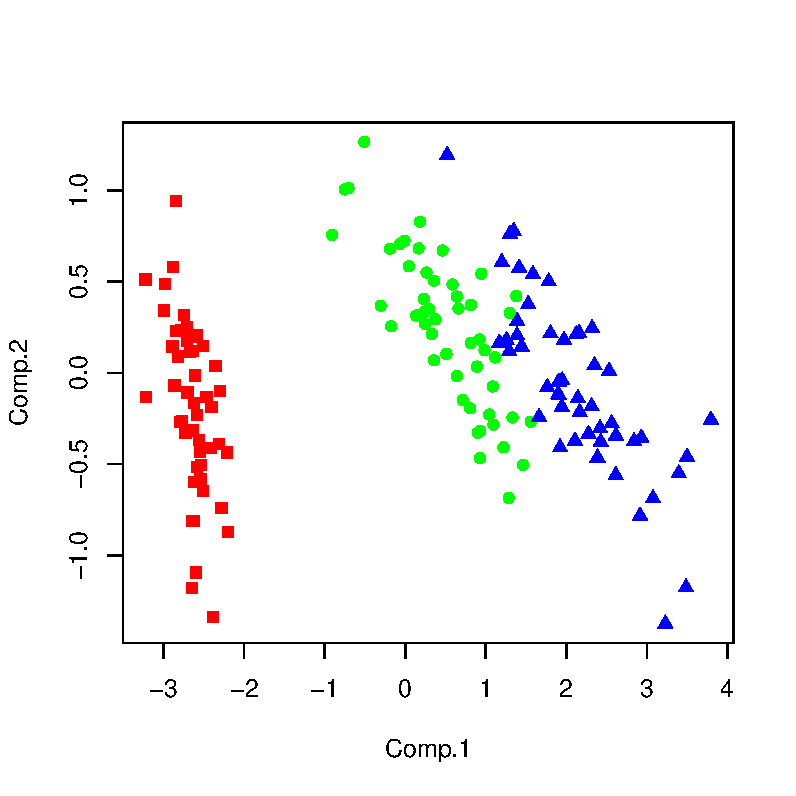
\includegraphics[width=0.425\textwidth]{figures/acp-iris.pdf}
%\caption{\label{fig:iris1}Représentation des Iris de Fisher dans le premier plan factoriel.}
\caption{\label{fig:iris1}Iris de Fisher, premier plan factoriel.}
\end{center}
\end{figure}

Comme nous l'avons écrit ci-dessus, on évitera les tableaux ou graphiques peu informatifs ou sans intérêt, qui polluent le document. Par exemple, pour comparer différentes populations en utilisant des diagrammes en boîte (\textit{boxplots}), on les juxtaposera dans la même figure. L'affichage des valeurs prises par une variable en fonction de l'indice des individus dans le jeu de données (figure~\ref{fig:iris2}), erreur trop souvent rencontrée dans les rapports, est typique de ce qu'il faut éviter. 

\begin{figure}[htbp]
\begin{center}
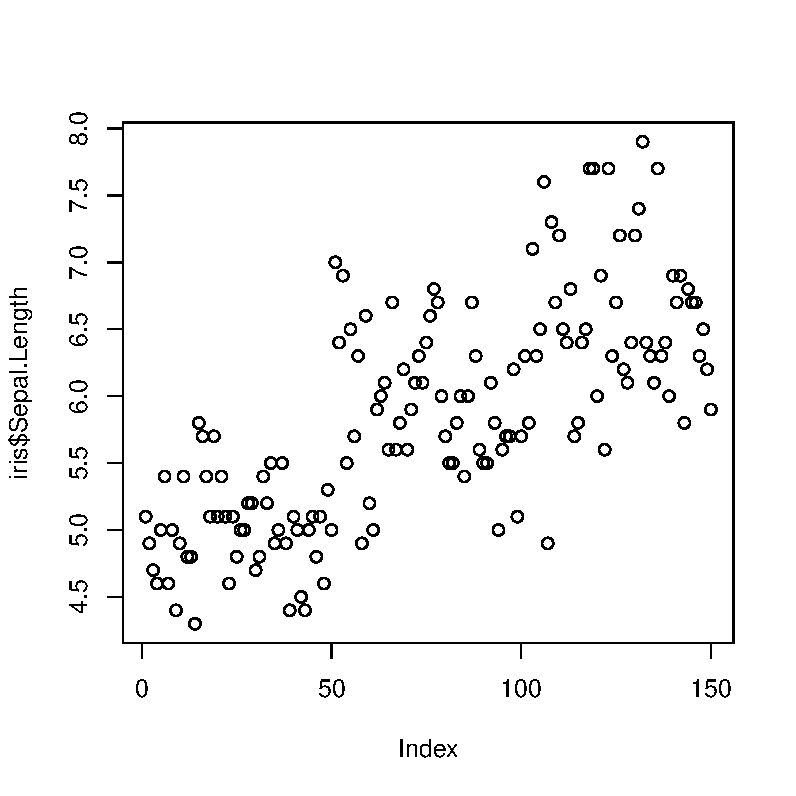
\includegraphics[width=0.425\textwidth]{figures/iris-seplen.pdf}
\caption{\label{fig:iris2}Figure pas optimisée: peu informative (abscisse sans intérêt), moche, sans couleur; à proscrire.}
\end{center}
\end{figure}


%------------------------------------------------

\subsection{Bibliographie}\label{subsec:CR:biblio}

C'est une partie parfois négligée, alors qu'elle est d'une importance fondamentale, puisqu'elle touche à la valorisation du travail et au problème du plagiat. L'intérêt de la bibliographie est de faire clairement référence aux connaissances antérieures (articles, livres, sites web, projets, code existant) à partir desquelles un travail est mené, et permet de positionner ce dernier par rapport à l'existant. Sans bibliographie, les contributions ne sont pas mises en valeur; et la paternité du travail présenté dans le document peut être remise en cause. 

Nous ne traiterons pas la question de la bibliographie en détails. Il existe en \LaTeX{}plusieurs possibilités. La solution la plus courante (et utilisée dans ce document), \BibTeX, nécessite de renseigner les références par type, dans un fichier à part (extension \verb?.bib?). La compilation du document se fait en plusieurs étapes. À chaque ajout d'une référence, il faudra ainsi compiler une fois avec \LaTeX, puis une fois avec \BibTeX, et enfin à nouveau une (voire deux) fois avec \LaTeX. 


%------------------------------------------------

\subsection{Conclusion}\label{subsec:CR:conclusion}

Ces conseils ont pour objectif de vous permettre de rédiger des documents plus agréables et faciles à lire. L'utilisation d'un logiciel tel que \LaTeX{} vous poussera à rédiger un compte-rendu avec rigueur, en sélectionnant et en structurant l'information que vous souhaitez restituer. Cette exigence n'est pas une perte de temps: elle sera profitable à la qualité de votre document, qui sera plus agréable à lire et à reprendre par la suite. 

Ce document ne dispense que des conseils élémentaires de rédaction et de mise en forme, et laisse de côté certains aspects jugés peu importants pour un rapport de projet. 
Il existe de nombreux documents permettant d'aller plus loin avec \LaTeX{} ou décrivant ses extensions (graphiques avec \verb?tikz?, diapositives avec \verb?Beamer?, etc): la littérature disponible est bien plus abondante que l'introduction générale \cite{oetiker18}. 


%------------------------------------------------

% Annexes éventuelles 

\appendix % la commande \appendix change la numérotation des paragraphes 

\section{\'Eléments sur la loi normale}\label{ann:gaus}

Voici un premier exemple d'appendice avec une définition (paragraphe~\ref{ann:gaus:def}) de la loi normale multivariée et une propriété de cette distribution relative au conditionnement (paragraphe~\ref{ann:gaus:cond}). 

\subsection{Définition}\label{ann:gaus:def}

La fonction de densité d'un vecteur aléatoire $\bsX$ distribué suivant une loi normale multivariée d'espérance $\mu$ et de matrice de covariance $\Sigma$ est \cite{petersen12} 
\begin{equation}
\displaystyle f_X(\bsx) = \frac{1}{(2\pi)^{\frac{p}{2}}|\bsSig|^{\frac{1}{2}}} \exp \left( \transp{(\bsx-\bsmu)} \bsSig^{-1} (\bsx-\bsmu) \right) , 
\end{equation}
où $\bsmu$ est un vecteur réel de dimensions $p \times 1$ et $\bsSig$ une matrice symétrique définie-positive de dimensions $p \times p$. 

\subsection{Propriété}\label{ann:gaus:cond}

\begin{propriete}[Loi normale et conditionnement]\label{pro:cond:gaus}
Soit $\bsX\sim\calN(\bsmu,\bsSig)$ un vecteur aléatoire gaussien (voir paragraphe \ref{ann:gaus:def}). Supposons que $\bsX$ peut être séparé en deux sous-vecteurs $\bsXa$ et $\bsXb$, où $A$ et  $B$ indiquent les indices des variables correspondantes: 
\begin{equation*}
\bsX = \left(\begin{array}{c} \bsXa \\ \bsXb \end{array}\right) , 
\bsmu = \left(\begin{array}{c} \bsmua \\ \bsmub \end{array}\right) , 
\bsSig = \left(\begin{array}{cc} \bsSigaa & \bsSigab \\ \bsSigba & \bsSigbb \end{array}\right) . 
\end{equation*}
Alors $\bsXa|\bsXb=\bsxb$ est un vecteur aléatoire gaussien: %more precisely, we have $\bsXa|\bsXo=\bsxo \ \follows{} \ \calN(\tilde{\bsmu},\tilde{\bsSig})$, with 
\begin{equation}
\label{eqn:condgaus1}
\bsXa|\bsXb=\bsxb \sim \calN(\bsmu_{A|B},\bsSig_{A|B}) , 
\end{equation}
où 
\begin{align*}
\label{eqn:condgaus2}
\bsmu_{A|B} & = \bsmua + \bsSigab \bsSigbb^{-1} (\bsxb-\bsmub) , \\ 
\bsSig_{A|B} & = \bsSigaa - \bsSigab \bsSigbb^{-1} \bsSigba . 
\end{align*}
\end{propriete}


%----------------------------------------------------------------------------------------

\bibliographystyle{abbrv}
\bibliography{Biblio}


\end{document}
